\chapter{流式主题模型算法设计}
\label{chapter:design}
大规模数据上的主题模型在国内外各大公司都得到了实现与应用,产生了重要的影响和价值。
流式数据环境下,主题模型的实现能够学习到主题的演化,并且动态地更新模型。
本章介绍了主题模型主要技术,并且提出了流式主题模型的设计。

\section{数学符号和术语}
本文通篇会使用到“词汇”,“文档”,“语料”,“主题”等术语。
比如,我们有时也会使用“隐变量”来表示用于标记抽象“主题”的变量。
为了避免这种歧义以及其他可能的问题,规范使用这些术语能够帮助描述和理解模型的设计。

如下,我们形式化地定义了一些术语与符号标记:
\begin{itemize}
\item 词汇:表示数据的基本单位,定义存在于一个词汇表中的元素。
\item 文档:表示为一个长度为$N$的词汇序列,$\mathbf{w}=(w_1, w_2, ..., w_N)$,其中$w_n$表示序列中的第$n$个词汇。
\item 语料:表示为一个大小为$M$的文档集合,$\mathbf{C=(w_1, w_2, ..., w_M)}$。
\item 主题:表示在文本预料集合$C$中语义内聚的多项式隐变量$z$。主题变量$z$的个数是一个有用户定义的常数$K$。
\item $\alpha, \eta$:表示Dirichlet模型的先验参数。
\item $\Theta, B$:表示LDA主题模型的后验参数。$\Theta=\mathbf{\{\theta_1, \theta_2, ...,\theta_M\}}$,
其中$\mathbf{\theta_m}$表示文档$\mathbf{w_m}$得到的主题分布。$B = \mathbf{ \{\beta_1, \beta_2, ...,\beta_K\}}$,
其中$\mathbf{\beta_k}$表示主题变量$z = k$的词汇分布。
\end{itemize}

\section{Latent Dirichlet Allocation(LDA)}
LDA的基本思路是将文档表示成主题随机变量的混合模型,每个主题表示为在词汇上的概率分布。
LDA提出的语料$C$文档生成过程描述如下:

0. 初始化参数$B$,$\{\beta_k \sim Dir(\eta_k)~ |~k \in [1, ... K]\}$

1. 从泊松分布中抽样第m篇文档的长度$N_m$,$N_m \sim Poisson(\xi)$

2. 从Dirichlet先验分布中抽样$\mathbf{\theta_m}$, $\mathbf{\theta_m} \sim Dir(\alpha_m)$

3. 抽样文档中的所有$N_m$个词项$w_n$:

~~~(a) 从多项式分布中抽样词项主题分配$z_n$,$z_n \sim Multinomial(\mathbf{\theta_m})$
   
~~~(b) 抽样一个词汇$w_n$,$w_n \sim p(w_n|\beta_{z_n})$

4. 对所有语料$C$中剩余的文档执行1 $\sim $ 3。\\
在上面的生成过程中,隐含着若干个假设:

(1) 给定主题模型的个数为$K$;

(2) 词生成概率矩阵$B$是一个$K \times V$的矩阵,$V$表示词汇表的大小;

(3) 每个文档的主题分布$\theta$都是$K$维的向量;

(4) 使用泊松分布作为文档长度的分布并不是决定的,如果有可以使用更好的分布;

(5) 文档长度$N$和其它主题模型的参数变量$\Theta, B, z$是相互独立的。\\
对于一个$K$维的Dirichlet变量$\mathbf{v}$落在一个$(K-1)$维的单纯形中(如果一个向量中的每个元素都不小于0,且总和为1,则落在$(K-1)$维的单存形中),
并且拥有如下概率密度:
\begin{equation}
Dir(\mathbf{v }| \mathbf{a} ) = \dfrac{\Gamma(\sum_{i=1}^K{a_i})}{\prod_{i=1}^K{\Gamma(a_i)}} 
v_1^{a_1-1} v_k^{a_k-1}
\end{equation}
其中,$\mathbf{a}$是一个$K$维的向量,且所有元素都大于0;$\Gamma(x)$表示Gamma函数。

Dirichlet函数对于单纯形来说是个简单的分布,它属于指数分布族,有有限的充分统计量。
Dirichlet还有一个重要的特性,这个特性便是和多项式分布式共轭。在许多应用中都会使用Dirichlet作为多项式分布的生成模型。

给定参数$\alpha, \eta$,参数$\Theta, B$,主题$\mathbf{z}$,数据$\mathbf{C}$的完全概率为:
\begin{equation}
p(\Theta, B, \mathbf{z, C} | \alpha, \eta) = \prod_{k=1}^K{Dir(\beta_k|\eta)}
\prod_{m=1}^M{\prod_{n=1}^N{Dir(\theta_m|\alpha)p(z_{mn}|\theta_m)p(w_{mn}|\beta_{z_{mn}})}}
\end{equation}
其中$p(z_{mn}|\theta_m)$表示主题取值为$z_mn$时的概率。通过积分,从上式可以得到数据集的概率:
\begin{equation}
p(\mathbf{C} | \alpha, \eta) = \prod_{k}^K{\prod_{m=1}^M{\int{Dir(\beta_k|\eta)} 
\int{Dir(\theta_m|\alpha)\prod_{n=1}^N{\sum_{z_{mn}}{p(z_{mn}|\theta_m)p(w_{mn}|\beta_{z_{mn}})}}}} d\theta_m }d\beta_k
\end{equation}

图\ref{fig:LDA}展示了LDA的概率图模型表示。图中$\theta_d$表示文档主题分布参数,$\beta_k$表示主题$z=k$的生成词概率分布。
$\alpha, \eta$分别表示LDA模型中文档主题分布$\theta_d$和主题生成词概率分布$\beta_k$的Dirichlet先验参数。
$z, w$表示每个文档中被采样生成的主题和词汇。

\begin{figure}[htb]\centering
  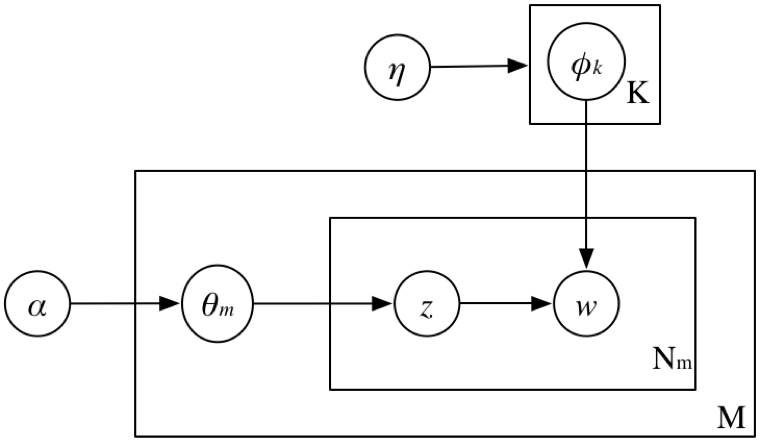
\includegraphics[width=0.5\linewidth]{LDA}
  \caption{LDA图模型表示}
  \label{fig:LDA}       % Give a unique label
\end{figure}

\subsection{批量LDA参数估计}
现有的LDA参数估计方法大多属于批量求解方法,主要包括两类算法,即变分方法和Gibbs采样。
前者的代表是Blei等人的VB方法\cite{blei2003latent}以及Teh等人的CVB\cite{teh2006a};
后者主要是Griffiths等人的CGBS\cite{griffiths2004finding}以及它的一些改进和扩展\cite{porteous2008fast, yao2009efficient, li2014reducing}。

在变分方法中,算法并非去直接估计真实的后验分布,而是借助另外一个更为简单的分布$q(z,\theta, \beta)$渐进地逼近正式的后验。
这些参数的最优值是通过最大化如下ELBO(Evidence Lower BOund, ELBO)得到的:
\begin{equation}
\log p(\mathbf{w} | \alpha, \eta) \ge L(\mathbf{w, \phi, \gamma, \lambda}) \triangleq 
\mathbb{E}_q{[\log p(\mathbf{w, z, \theta, \beta} | \alpha, \eta)]} - 
\mathbb{E}_q{[\log q(\mathbf{z, \theta, \beta})]}.
\end{equation}
其中$\phi, \gamma, \lambda$是变分方法引入变分参数,$\gamma$和$\lambda$分别是变分方法中$\theta$和$\beta$的Dirichlet先验。
值得强调的是,这里最大化ELBO等价于最小化分布$q(\mathbf{z, \theta, \beta})$和后验分布$p(\mathbf{z, \theta, \beta} | \mathbf{w}, \alpha, \eta)$之间的KL距离。

\begin{algorithm}[htb]  
\caption{ Batch Variational Bayes for LDA} 
\label{alg:bvb} 
\begin{algorithmic}[1] 
\Require Corpus $\mathbf{C = \{w_1, w_2, ..., w_M\}}$
\State Random initialize parameter $\lambda$
\While {relative improvement in $L(\mathbf{w, \phi, \gamma, \lambda}) > 0.00001$}
\State E step:
\For { m = 1 to M }
\State Set $\gamma_{mk} = 1$
\Repeat
\State Update $\phi_{mwk}, \gamma_{mk} $
\Until{ change in $\gamma_{mk} $ is relative small}
\EndFor
\State M step:
\State Update $\lambda_{kw}$
\EndWhile
\end{algorithmic}  
\end{algorithm}  

根据VB方法,可以得到上面的批量变分参数优化算法。

Gibbs采样算法是另一种主要LDA参数估计方法,并且更易于实现,因而在许多算法实现中得到了应用\cite{Liu:2011:PPL:1961189.1961198, Peacock, li2014scaling}。 

Gibbs采样算法(GiBbs Sampling)是马可夫蒙特卡洛(Markov-chain Monte Carlo, MCMC)算法的一种特例\cite{mackay2002information, hesterberg2012monte}。
MCMC算法的主要思路是构造一个非周期马氏链,并按照某一个转移概率反复地对马氏链的各个状态进行抽样,最终马氏链的状态分布会收敛于一个稳定的分布$\pi$。
虽然,我们无法直接获知$\pi$的具体值,但是我们仍然能够从分布中得到样本。
按照这种定义,只需要从分布中获取得到足够多的样本便可以很快地计算出稳定分布的近似估计$\hat{\pi}$。

\begin{figure}[htb]\centering
  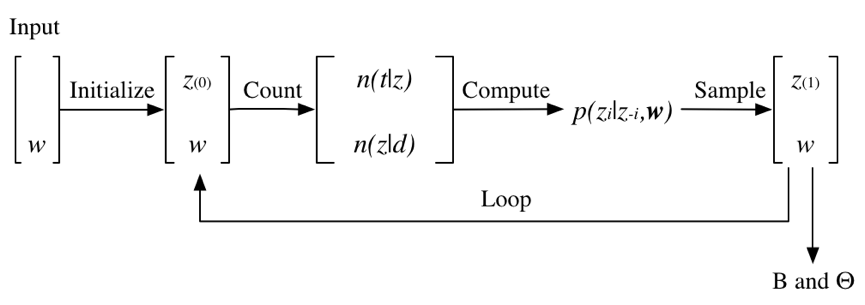
\includegraphics[width=0.8\linewidth]{Gibbs_Sampling}
  \caption{使用Gibbs采样算法学习LDA过程}
  \label{fig:Gibbs_Sampling}       % Give a unique label
\end{figure}

CGBS算法中提出的Gibbs采样算法通过积分消除了模型参数$\theta, \beta$,使得算法相比于直接的GBS算法能够更快地收敛:
\begin{equation}
\label{eq:pzw}
\begin{aligned}
p(\mathbf{z , w | \alpha, \eta}) &= p(\mathbf{w | z , \alpha, \eta}) p(\mathbf{z| \alpha, \eta}) \\
p(\mathbf{w | z, \alpha, \eta})                &= \left( \dfrac{\Gamma(V\eta)}{\Gamma(\eta)^V} \right)^K
\prod_{k=1}^K{\dfrac{ \prod_w^V \Gamma( n_{k,w} + \eta )}{\Gamma( n_{k, \cdot}+ V \eta)}} \\
p(\mathbf{z | \alpha, \eta})                    &=\left( \dfrac{\Gamma(K\alpha)}{\Gamma(\alpha)^K} \right)^M
\prod_{m=1}^M{\dfrac{ \prod_k^K \Gamma( n_{k,m} + \alpha)}{\Gamma( n_{\cdot, m}+ K \alpha)}} \\
\end{aligned}
\end{equation}
其中,$n_{k,w}$表示语料中词汇$w$的主题分配为$z=k$的计数,$n_{k, m}$表示文档中主题分配为$z=k$的词项的计数。
$n_{k, \cdot} = \sum_w^V{n_{k, w}} , n_{\bullet, m} = \sum_k^K{ n_{k, m}}$。

\begin{algorithm}[htb]
\caption{ Batch Collapsed Gibbs Sampling for LDA} 
\label{alg:bcgbs}
\begin{algorithmic}[1] 
\Require Corpus $\mathbf{C = \{w_1, w_2, ..., w_M\}}$
\State Random assign topic to each word in $\mathbf{C}$
\State Collect and summary $n_{k, w}$ and $n_{k, m}$
\While {Not converged or iter > MAX\_ITERATION}
\For { m = 1 to $M$ }
\For { n = 1 to $N_m$}
\State Sample $z_{mn} \sim p(z_{mn} | \mathbf{z}_{\neg (mn)}, \mathbf{w}) $
\State Update  $n_{k, w}$ and $n_{k, m}$ according to $z_{mn}$
\EndFor
\EndFor
\EndWhile
\end{algorithmic}  
\end{algorithm}  

借助式子\ref{eq:pzw},可以得到下面的抽样分布的定义:
\begin{equation}
\begin{aligned}
p( z_i = k | \mathbf{z}_{\neg i},  \mathbf{w}) 
&\propto p( z_i = k , w_i = t | \mathbf{z}_{\neg i}, \mathbf{w}_{\neg i}) \\
& = \dfrac{p(\mathbf{w |z}) p(\mathbf{z})}{p(\mathbf{w}_{\neg i} | \mathbf{z}_{\neg i})p(\mathbf{z}_{\neg i})} \\
& = \dfrac{ n_{k, w_i}^{\neg i,j} + \eta }{ n_{k, \cdot}^{\neg i,j} + V\eta}
\dfrac{n_{k, m}^{\neg i,j} + \alpha}{n_{\cdot, m}^{\neg i,j} + K \alpha}
\end{aligned} 
\end{equation}
其中$n^{\neg i,j}$表示不包括$z_i$的计数。这个抽样分布的式子很直观,
左边其实主题生成词概率的Dirichlet后验估计,右边则是文档主题分布的Dirichlet后验估计,正好反映了LDA模型先抽样主题,然后再抽样根据主题抽样词汇的生成过程。

算法\ref{alg:bcgbs}展示了批量CGBS的算法学习过程。
算法首先随机为语料中的每个词项分配一个主题,并统计$n_{k, w}$和$n_{k, m}$的值。
之后算法按照类似坐标轴下降的方法,顺序地抽样语料中的每个词汇的主题。
每个迭代将会遍历语料中所有的文档的所有词项。若干次迭代之后算法,最终会收敛。
值得注意的是,这边坐标轴下降方法中并不一定需要顺序地抽样语料中的每个词汇,实际上词汇之间先后的抽样顺序并不相关,可以按照任意顺序进行抽样。

批量的算法是LDA模型求解算法的主流算法,在语料大小可以完全被加载时,这种算法具有实现简单更加精确的优点。然而在数据量太大,数据分布不稳定的情况下,在线算法往往体现出来更好的性能。

\subsection{在线LDA参数估计}
\begin{algorithm}[htb]
\caption{Online Variational Bayes for LDA} 
\label{alg:olda}
\begin{algorithmic}[1] 
\State Define $\rho_t \triangleq (\tau_0 + t)^{-\kappa}$
\State Random initialize parameter $\lambda$
\For{ t = 0 to $\infty$}
\State E step:
\State Set $\gamma_{tk} = 1$
\Repeat
\State Update $\phi_{twk}, \gamma_{tk} $
\Until{ change in $\gamma_{tk} $ is relative small}
\State M step:
\State Update $\tilde{\lambda}_{kw}$
\State Set $\mathbf{\lambda}=(1- \rho_t) \mathbf{\lambda} + \rho_t \tilde{\mathbf{\lambda}}$
\EndFor
\end{algorithmic}  
\end{algorithm}  

在标准批量学习方法中,算法每一轮迭代都需要遍历整个数据集,这种计算方法带来的资源消耗非常高。
特别在主题模型应用中,这种现象更为常见——主题模型往往需要借助大规模的数据集上训练,
来挖掘人为无法标记的主题。虽然,使用分布式并行也能解决这种数据规模大的问题,但是这并不妨碍人们提出LDA参数估计的在线模型。

OLDA(Online Latent Dirichlet Allocation, OLDA)\cite{hoffman2010online}提出的在线VB方法将主题模型看作概率矩阵分解,并参考在线矩阵分解的技术\cite{mairal2010online},提出了如下在线算法\ref{alg:olda}。

算法\ref{alg:olda}中,语料集视为无穷大,并且按照时间分片一次一小批次地输入,所有词汇$w$来自于固定的词汇集$V$。
在整个算法执行过程中,$\lambda$起到了重要的作用,在这里$\lambda$参数表示LDA模型$\beta$的变分Dirichlet后验参数。随着时间的推移,$t$时刻之前的$\lambda$并没有被丢弃,而是通过一种衰减的方式保留下来。

衰减的权重设计为$\rho_t \triangleq (\tau_0 + t ) ^{-\kappa}$,这个式子中$\kappa \in (0.5, 1], \tau \ge 0$。
这么做的好处就是不断会有新的后验知识加入进来,并且旧的先验知识和后验知识的比例关系得到协调(时间越靠前的权重越小),使得模型在对全局的知识都有很好的掌握,,并很快地收敛。

On-Line LDA\cite{alsumait2008on-line}算法则从Gibbs采样算法的角度出发设计了在线LDA算法。

\begin{algorithm}[htb]
\caption{Online Gibbs Sampling for LDA} 
\label{alg:on-linelda}
\begin{algorithmic}[1]
\Require $ a, b, \omega^{\sigma}, S^t, t \in [1, +\infty)$
\For{ t = 1 to $\infty$}
\If{t == 1}
\State $\eta_k^t = b, k \in \{1, ..., K\}$
\Else
\State $\eta_k^t = B_k^{t-1} \omega^{\sigma}, k \in \{1, ..., K\}$
\EndIf
\State Random assign topic to each word in $S^t$
\For{ each word $w$ in $S^t$ }
\State GibbsSampling($S^t, \eta^{t - 1}, \alpha$)
\EndFor
\State Collect and summary $n_{k,w}^{(t)}$和$n_{k}^{(t)}$
\State Set $\beta_{k,w}^{(t)} = n_{k,w}^{(t)}$
\State Set $B_k^t = B_k^{t - 1} \cup \beta_k^{(t)}$
\EndFor
\end{algorithmic}  
\end{algorithm}  

算法\ref{alg:on-linelda}中,$\omega$是一个维度为$\sigma \time 1 $的向量,表示了时刻$t$之前的$\sigma$时刻内的$\beta$在先验中所占的权重。$\beta_k^t$是在$t$时刻词汇与主题$k$共现计数,是一个维度为$V^t \times 1$的向量。
$B_k^t$是一个$V^t \times \sigma$的演变矩阵。

通过这种窗口化的机制,算法不仅能够快速收敛,还能使得模型更聚焦于最近的数据。
对于那些时间太久远的潜在语义则有可能被遗忘,因而能够更精确地捕获主题在时间轴上的演变。
On-Line LDA借此将主题模型很好地应用于主题检测与跟踪。

\section{流式主题模型算法} 
流式数据带有显著的特性:无限性、无序性、突发性、易失性和实时性。
互联网社交网络和自媒体的广泛应用和发展,使得文本数据的增长速度越来越快。
并且网络上热议的话题经常因为各种现实世界的环境或者突发因素而改变(比如季节、社会事件等等),并且带有强烈的话题时效性。
\begin{figure}[htb]\centering
  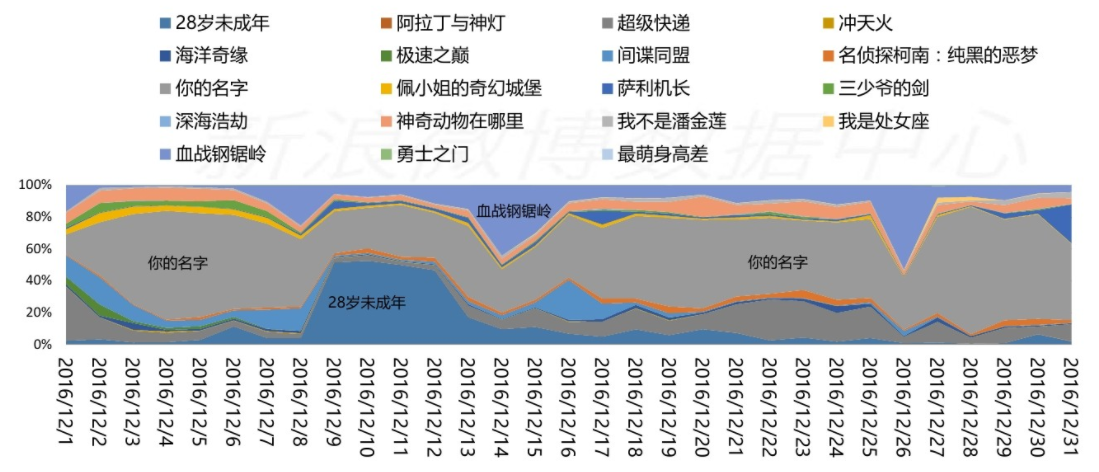
\includegraphics[width=1\linewidth]{movie-hot}
  \caption{2016年12月在映电影微博热议度变化趋势}
  \label{fig:LDA}       % Give a unique label
\end{figure}

对于此类数据,不仅内容演变快,同一时刻到达的数据量也非常可观。
大多数据公司都会采用分布式流式处理引擎来保证高吞吐率,高速率的数据处理。
常见的分布式流式计算引擎包括Storm,Spark Streaming和Samza。

可见海量的数据,频繁演变的主题趋势是一个很现实的问题。
如果仍然使用批量的算法来训练主题模型,那么在应用中不得不频繁地重新训练模型。
显然这种方法代价高昂,并且未必能够很好地利用所有的数据以及捕获主题的演变。
在线算法可以对主题演变进行良好的建模,但是目前的算法并没有提出大规模的分布式流式数据上的在线主题模型算法。

考虑到P.Domingos和G.Hulten\cite{Domingos01catchingup}提出
的数据流算法应该具有的特性:

(1) 对每个数据样本只需要很少的运算时间

(2) 使用内存大小固定,与处理的样本数据总量无关

(3) 在构建模型的过程中,所有训练数据只会被计算一遍或少数几遍

(4) 随时产生独立于样本顺序的模型

(5) 具有概念迁移能力。

本文提出了如下两种分布式流式数据算法框架,在线流式主题模型和增量流式主题模型。

\subsection{在线流式主题模型}
在线流式主题模型的提出主要是受到了OLDA\cite{hoffman2010online}和On-Line LDA\cite{alsumait2008on-line}的启发。
这两个算法都将数据集进行时间分片,但是每个时间片只会有一篇文档出现。
这种一个时间分片一篇文档的串行做法无法直接扩展到流式主题模型应用之上。
本文的做法是对数据集进行时间分片,但是每个时间分片内都包含若干篇文档。
当某一时间片的数据集到达时,应用便会通过分布式并行的Gibbs采样算法更新模型,并产生必要的输出。

分布式并行Gibbs采样算法的提出参考了\cite{smola2010an}。在分布式算法中,数据被均衡地分布式存储在不同的位置,因而并行算法可以通过数据并行的方式实现。考虑到:
\begin{equation}
p( z_i = k | \mathbf{z}_{\neg i},  \mathbf{w}) 
 \propto \dfrac{ n_{k, w_i}^{\neg i,j} + \eta }{ n_{k, \cdot}^{\neg i,j} + V\eta}
(n_{k, m}^{\neg i,j} + \alpha)
\end{equation}
主题抽样的概率只会依赖于$n_{k, w_i}^{\neg i,j}, n_{k, \cdot}^{\neg i,j}, n_{k, m}^{\neg i,j}$,因而与其他文档的主题计数无关。
主题模型并行采样算法的核心思想便是少数文档的采样并不会对全局主题分布$n(k)$和词汇-主题表$n(w, k)$造成很大的影响。
这意味着并行算法可以放松对$n(k)$和$n(w, k)$的同步(严格的同步极大的降低分布式算法的效率),从而可以加大算法的并行度同时保证算法收敛。
综上,本文提出的算法将设置$n(k)$和$n(w, k)$为全局参数,并假设在某些时刻这两个参数会得到同步(比如,以时间片为粒度)。
\begin{algorithm}[]
\caption{Online Stream Topic Model}
\label{alg:onlineStreamLDA}
\textbf{\underline{Task Scheduler:}}
\begin{algorithmic}[1]
\Function{UPDATE\_VOCAB\&PARAMS}{$t$}
\State Collect and summary vocabulary $V^t$ at $S^t$
\State Add unkown words to $V_g$, $V_g = V_g \cup V^t$
\State Set $\beta^t(w, k) = \eta$, push $\beta^t(w, k)$, for $w \in (V_g - V^t)$, and update $\beta^t(k)$ accordingly.
\State Synchronize and pull parameter set $\beta^t(k), \beta^t(w, k)$ from servers
\State Set $\bigtriangleup \beta^t(k) = (\rho_t - 1) \beta^t(k), \bigtriangleup \beta^t(w, k) = (\rho_t - 1) \beta^t(w, k)$
\State Push $\bigtriangleup \beta^t(k), \bigtriangleup \beta^t(w, k)$  to servers and synchronize.
\EndFunction
\State Create a global vocabulary $V_g$
\For{ t = 1 to $\infty$}
\State Issue UPDATE\_VOCAB\&PARAMS(t)
\State Issue WORKER\_SAMPLE($t$) to all workers
\EndFor
\end{algorithmic}
\textbf{\underline{Workers $r = 1, ..., R$:}}
\begin{algorithmic}[1]
\Function{ LOAD\_DATA}{$t$}
\State Load a part of training data of $S^t$ as $C^t$
\State Pull the parameter set $\beta^t(k)$ and $\beta^t(w, k)$ from servers
\EndFunction
\Function{ WORKER\_SAMPLE}{$t$}
\State Issue LOAD\_DATA($t$)
\State Initialize topic assignment to each word in $C^t$ 
\For{ each word $w$ in $C^t$ }
\State DO\_SAMPLING($C^t, \beta^t(k), \beta^t(w, k), \alpha$)
\EndFor
\State Collect and summary $n_{k,w}^{(t)}$ and $n_{k}^{(t)}$
\State Set $\bigtriangleup \beta^t(k) = \rho_t n_{k}^{(t)}, \bigtriangleup \beta^t(w, k) = \rho_t n_{k,w}^{(t)}$ and push $\bigtriangleup \beta^t(k), \bigtriangleup \beta^t(w, k)$ to servers
\EndFunction
\end{algorithmic}  
\textbf{\underline{Servers:}}
\begin{algorithmic}[1]
\Function{SERVER\_ITERATE}{$t$}
\State Aggregate $\bigtriangleup \beta^t(k) = \sum_r^R{\bigtriangleup \beta^t_r(k)}, \bigtriangleup \beta^t(w, k) = \sum_r^R{\bigtriangleup \beta^t_r(w, k)}$
\State $\beta^{(t+1)}(k) =\beta^t(k) +  \bigtriangleup \beta^t(k), \beta^{(t+1)}(w, k) = \beta^t(w, k) + \bigtriangleup \beta^t(w, k)$
\EndFunction
\end{algorithmic}
\end{algorithm}  

算法\ref{alg:onlineStreamLDA}总共分为三个部分Task Scheduler, Workers, Servers。其中Task Scheduler是一个单机的算法调度模块,Workers是分布式并行的主要进程,Servers表示参数服务器。$\rho_t \in (0, 1)$表示衰减权重,可以有不同的定义。
这么做使得$\beta^t(k)$和$\beta^t(w, k)$拥有历史信息。
根据Dirichlet和多项式分布共轭的属性,我们将已观测到$\beta^t(w, k)$信息作为主题生成词多项式分布的Dirichlet先验。FastGibbsSampling函数提供了快速地采样算法,本文将这一部分放在后面的章节讨论。

流式主题模型算法迭代以时间为单位,在每个Worker的采样算法开始之前,各个Worker得到的模型参数是同步的。
而在每个时间片内部,所有的Worker之间是完全异步的,Worker进程之间的采样过程不需要互相等待。
另外在流式环境下,不断会有新词出现,模型必须能够动态的维护新词。
这种新词所带来的维护成本巨大,本文将在后面的章节中对此进行讨论分析。

\subsection{增量流式主题模型}
%增量学习方法的思路来自于\cite{Canini_onlineinference}
除了上一节提到的使用衰减权重的方法来保留历史信息,并使得模型更容易演变。
本节介绍的算法采用窗口化的方法,在流数据移动窗口,窗口内的所有数据信息将会被保留,窗口外的所有数据信息将会被消除。
显然,窗口越大模型所能保留的数据信息越完整。当窗口足够大时,我们有理由相信模型算法能够训练得到一个趋近与真实数据分布的模型。

\begin{algorithm}
\caption{Incremental Stream Topic Model}
\label{alg:IncStreamLDA}
\textbf{\underline{Task Scheduler:}}
\begin{algorithmic}[1]
\Function{UPDATE\_VOCAB\&PARAMS}{$t$}
\State Collect and summary vocabulary $V^t$ at $S^t$
\State Add unkown words to $V_g$, $V_g = V_g \cup V^t$
\EndFunction
\State Create a global vocabulary $V_g$
\For{ t = 1 to $\infty$}
\State Issue UPDATE\_VOCAB\&PARAMS(t)
\State Issue WORKER\_SAMPLE($t$) to all workers
\EndFor
\end{algorithmic}
\textbf{\underline{Worker $r = 1, ..., R$:}}
\begin{algorithmic}[1]
\Function{ LOAD\_DATA}{$t$}
\State Load a part of training data of $S^t$ as $C^t$
\State Pull the parameter set $\beta^t(k)$ and $\beta^t(w, k)$ from servers
\EndFunction
\Function{ WORKER\_SAMPLE}{$t$}
\State Issue LOAD\_DATA($t$)
\State Initialize topic assignment to each word in $C^t$ 
\For{ each word $w$ in $C^t$ }
\State DO\_SAMPLING($C^t, \beta^t(k), \beta^t(w, k), \alpha$)
\EndFor
\State Collect and summary $n_{k,w}^{(t)}$ and $n_{k}^{(t)}$
\State Load $\bigtriangleup \beta^{t - \sigma}(k), \bigtriangleup \beta^{t - \sigma}(w, k)$ from local file
\State Set $\bigtriangleup \beta^t(k) = n_{k}^{(t)} - \beta^{t - \sigma}(k), \bigtriangleup \beta^t(w, k) = n_{k,w}^{(t)} - \beta^{t - \sigma}(w, k)$ 
\State Push $\bigtriangleup \beta^t(k), \bigtriangleup \beta^t(w, k)$ to servers
\State Store $\bigtriangleup \beta^t(k), \bigtriangleup \beta^t(w, k)$ to local file
\EndFunction
\end{algorithmic}
\textbf{\underline{Servers:}}
\begin{algorithmic}[1]
\Function{SERVER\_ITERATE}{$t$}
\State Aggregate $\bigtriangleup \beta^t(k) = \sum_r^R{\bigtriangleup \beta^t_r(k)}, \bigtriangleup \beta^t(w, k) = \sum_r^R{\bigtriangleup \beta^t_r(w, k)}$
\State $\beta^{(t+1)}(k) =\beta^t(k) +  \bigtriangleup \beta^t(k), \beta^{(t+1)}(w, k) = \beta^t(w, k) + \bigtriangleup \beta^t(w, k)$
\EndFunction
\end{algorithmic}
\end{algorithm}  

使用窗口机制的另外一个好处在于能够使得模型更聚焦于近段时间的数据,从而学习到更具有时效性的模型。
另外,窗口机制还存在其他优点本文将在后续章节讨论。

算法\ref{alg:IncStreamLDA}与算法\ref{alg:onlineStreamLDA}相同具有三个部分,与其不同之处在于算法\ref{alg:IncStreamLDA}不使用衰减权重来保留历史信息,
而是保留窗口$[t - \sigma, t]$内的所有时间片的词汇-主题计数信息。这种方法从实现上来说更简单,也会带来更多的优点,在后续的章节中将予以讨论。
\section{本章小结}
本章主要介绍了大规模流式主题模型的设计。首先介绍了LDA模型的基本理论背景,包括LDA模型的介绍,以及常见LDA参数估计方法。从算法框架角度看,又有多种不同的批量估计方法和在估计方法。
在流式数据环境下,数据呈现出海量、高速、实时等特性。这些特性使得批量算法和简单的在线算法无法被直接应用。
因此,本文提出了两种大规模流式主题模型的设计方案,分别是在线流式主题模型和增量流式主题模型。在后续的章节中,本文将更加详细地介绍如何高效地实现这两类流式主题模型算法。
